\chapter{Conceptos básicos de grafos}

Muchos problemas de programación se pueden resolver
modelando el problema como un problema de grafo
y utilizando un algoritmo de grafo adecuado.
Un ejemplo típico de grafo es una red
de carreteras y ciudades en un país.
A veces, sin embargo, el grafo está oculto
en el problema y puede ser difícil de detectarlo.

Esta parte del libro discute los algoritmos de grafos,
especialmente centrándose en temas que
son importantes en la programación competitiva.
En este capítulo, repasamos conceptos
relacionados con grafos,
y estudiamos diferentes formas de representar grafos en algoritmos.

\section{Terminología de grafos}

\index{grafo}
\index{nodo}
\index{arista}

Un \key{grafo} consta de \key{nodos}
y \key{aristas}. En este libro,
la variable $n$ denota el número de nodos
en un grafo, y la variable $m$ denota
el número de aristas.
Los nodos están numerados
usando números enteros $1,2,\ldots,n$.

Por ejemplo, el siguiente grafo consta de 5 nodos y 7 aristas:

\begin{center}
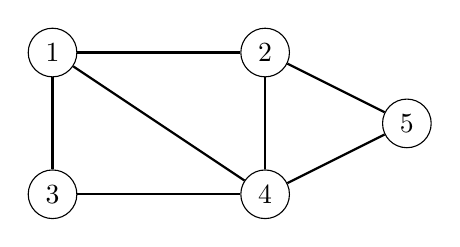
\begin{tikzpicture}[scale=0.9]
\node[draw, circle] (1) at (1,3) {$1$};
\node[draw, circle] (2) at (4,3) {$2$};
\node[draw, circle] (3) at (1,1) {$3$};
\node[draw, circle] (4) at (4,1) {$4$};
\node[draw, circle] (5) at (6,2) {$5$};

\path[draw,thick,-] (1) -- (2);
\path[draw,thick,-] (1) -- (3);
\path[draw,thick,-] (1) -- (4);
\path[draw,thick,-] (3) -- (4);
\path[draw,thick,-] (2) -- (4);
\path[draw,thick,-] (2) -- (5);
\path[draw,thick,-] (4) -- (5);
\end{tikzpicture}
\end{center}

\index{camino}

Un \key{camino} va del nodo $a$ al nodo $b$
a través de aristas del grafo.
La \key{longitud} de un camino es el número de
aristas en él.
Por ejemplo, el grafo anterior contiene
un camino $1 \rightarrow 3 \rightarrow 4 \rightarrow 5$
de longitud 3
desde el nodo 1 al nodo 5:

\begin{center}
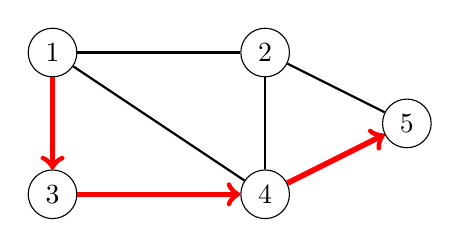
\begin{tikzpicture}[scale=0.9]
\node[draw, circle] (1) at (1,3) {$1$};
\node[draw, circle] (2) at (4,3) {$2$};
\node[draw, circle] (3) at (1,1) {$3$};
\node[draw, circle] (4) at (4,1) {$4$};
\node[draw, circle] (5) at (6,2) {$5$};

\path[draw,thick,-] (1) -- (2);
\path[draw,thick,-] (1) -- (3);
\path[draw,thick,-] (1) -- (4);
\path[draw,thick,-] (3) -- (4);
\path[draw,thick,-] (2) -- (4);
\path[draw,thick,-] (2) -- (5);
\path[draw,thick,-] (4) -- (5);

\path[draw=red,thick,->,line width=2pt] (1) -- (3);
\path[draw=red,thick,->,line width=2pt] (3) -- (4);
\path[draw=red,thick,->,line width=2pt] (4) -- (5);
\end{tikzpicture}
\end{center}

\index{ciclo}

Un camino es un \key{ciclo} si el primer y último
nodo es el mismo.
Por ejemplo, el grafo anterior contiene
un ciclo $1 \rightarrow 3 \rightarrow 4 \rightarrow 1$.
Un camino es \key{simple} si cada nodo aparece
a lo sumo una vez en el camino.


% 
% \begin{itemize}
% \item $1 \rightarrow 2 \rightarrow 5$ (length 2)
% \item $1 \rightarrow 4 \rightarrow 5$ (length 2)
% \item $1 \rightarrow 2 \rightarrow 4 \rightarrow 5$ (length 3)
% \item $1 \rightarrow 3 \rightarrow 4 \rightarrow 5$ (length 3)
% \item $1 \rightarrow 4 \rightarrow 2 \rightarrow 5$ (length 3)
% \item $1 \rightarrow 3 \rightarrow 4 \rightarrow 2 \rightarrow 5$ (length 4)
% \end{itemize}

\subsubsection{Conectividad}

\index{grafo conectado}

Un grafo es \key{conectado} si hay un camino
entre cualquier par de nodos.
Por ejemplo, el siguiente grafo está conectado:
\begin{center}
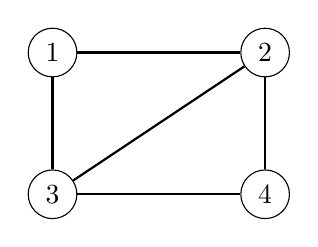
\begin{tikzpicture}[scale=0.9]
\node[draw, circle] (1) at (1,3) {$1$};
\node[draw, circle] (2) at (4,3) {$2$};
\node[draw, circle] (3) at (1,1) {$3$};
\node[draw, circle] (4) at (4,1) {$4$};
\path[draw,thick,-] (1) -- (2);
\path[draw,thick,-] (1) -- (3);
\path[draw,thick,-] (2) -- (3);
\path[draw,thick,-] (3) -- (4);
\path[draw,thick,-] (2) -- (4);
\end{tikzpicture}
\end{center}

El siguiente grafo no está conectado,
porque no es posible llegar
desde el nodo 4 a cualquier otro nodo:
\begin{center}
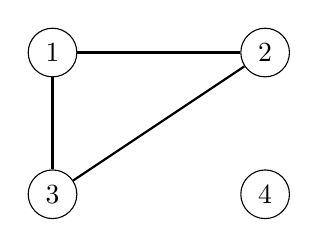
\begin{tikzpicture}[scale=0.9]
\node[draw, circle] (1) at (1,3) {$1$};
\node[draw, circle] (2) at (4,3) {$2$};
\node[draw, circle] (3) at (1,1) {$3$};
\node[draw, circle] (4) at (4,1) {$4$};
\path[draw,thick,-] (1) -- (2);
\path[draw,thick,-] (1) -- (3);
\path[draw,thick,-] (2) -- (3);
\end{tikzpicture}
\end{center}

\index{componente}

Las partes conectadas de un grafo son
llamadas sus \key{componentes}.
Por ejemplo, el siguiente grafo
contiene tres componentes:
$\{1,\,2,\,3\}$,
$\{4,\,5,\,6,\,7\}$ y
$\{8\}$.
\begin{center}
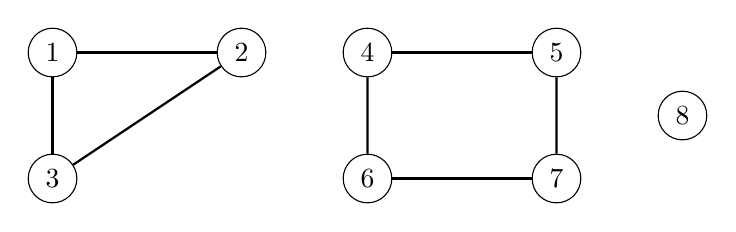
\begin{tikzpicture}[scale=0.8]
\node[draw, circle] (1) at (1,3) {$1$};
\node[draw, circle] (2) at (4,3) {$2$};
\node[draw, circle] (3) at (1,1) {$3$};

\node[draw, circle] (6) at (6,1) {$6$};
\node[draw, circle] (7) at (9,1) {$7$};
\node[draw, circle] (4) at (6,3) {$4$};
\node[draw, circle] (5) at (9,3) {$5$};

\node[draw, circle] (8) at (11,2) {$8$};

\path[draw,thick,-] (1) -- (2);
\path[draw,thick,-] (2) -- (3);
\path[draw,thick,-] (1) -- (3);
\path[draw,thick,-] (4) -- (5);
\path[draw,thick,-] (5) -- (7);
\path[draw,thick,-] (6) -- (7);
\path[draw,thick,-] (6) -- (4);
\end{tikzpicture}
\end{center}

\index{árbol}

Un \key{árbol} es un grafo conectado
que consta de $n$ nodos y $n-1$ aristas.
Hay un camino único
entre cualquier par de nodos de un árbol.
Por ejemplo, el siguiente grafo es un árbol:

\begin{center}
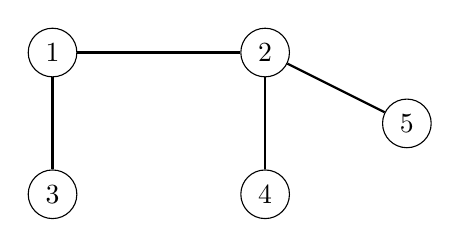
\begin{tikzpicture}[scale=0.9]
\node[draw, circle] (1) at (1,3) {$1$};
\node[draw, circle] (2) at (4,3) {$2$};
\node[draw, circle] (3) at (1,1) {$3$};
\node[draw, circle] (4) at (4,1) {$4$};
\node[draw, circle] (5) at (6,2) {$5$};

\path[draw,thick,-] (1) -- (2);
\path[draw,thick,-] (1) -- (3);
%\path[draw,thick,-] (1) -- (4);
\path[draw,thick,-] (2) -- (5);
\path[draw,thick,-] (2) -- (4);
%\path[draw,thick,-] (4) -- (5);
\end{tikzpicture}
\end{center}

\subsubsection{Direcciones de las aristas}

\index{grafo dirigido}

Un grafo es \key{dirigido}
si las aristas se pueden recorrer
solo en una dirección.
Por ejemplo, el siguiente grafo es dirigido:
\begin{center}
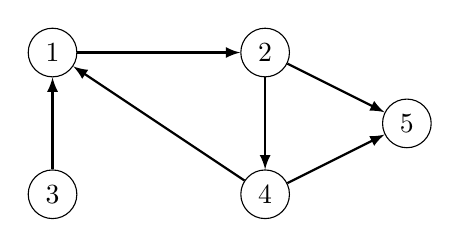
\begin{tikzpicture}[scale=0.9]
\node[draw, circle] (1) at (1,3) {$1$};
\node[draw, circle] (2) at (4,3) {$2$};
\node[draw, circle] (3) at (1,1) {$3$};
\node[draw, circle] (4) at (4,1) {$4$};
\node[draw, circle] (5) at (6,2) {$5$};
\path[draw,thick,->,>=latex] (1) -- (2);
\path[draw,thick,->,>=latex] (2) -- (4);
\path[draw,thick,->,>=latex] (2) -- (5);
\path[draw,thick,->,>=latex] (4) -- (5);
\path[draw,thick,->,>=latex] (4) -- (1);
\path[draw,thick,->,>=latex] (3) -- (1);
\end{tikzpicture}
\end{center}

El grafo anterior contiene
un camino $3 \rightarrow 1 \rightarrow 2 \rightarrow 5$
desde el nodo $3$ hasta el nodo $5$,
pero no hay un camino desde el nodo $5$ hasta el nodo $3$.

\subsubsection{Pesos de las aristas}

\index{grafo con pesos}

En un \key{grafo con pesos}, a cada arista se le asigna
un \key{peso}.
Los pesos a menudo se interpretan como longitudes de arista.
Por ejemplo, el siguiente grafo es con pesos:
\begin{center}
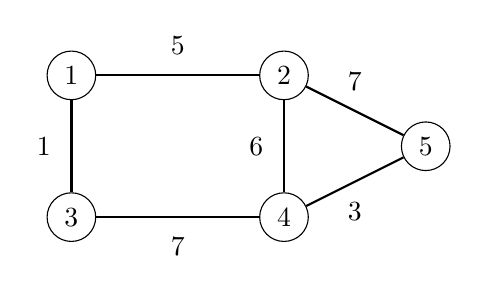
\begin{tikzpicture}[scale=0.9]
\node[draw, circle] (1) at (1,3) {$1$};
\node[draw, circle] (2) at (4,3) {$2$};
\node[draw, circle] (3) at (1,1) {$3$};
\node[draw, circle] (4) at (4,1) {$4$};
\node[draw, circle] (5) at (6,2) {$5$};
\path[draw,thick,-] (1) -- node[font=\small,label=above:5] {} (2);
\path[draw,thick,-] (1) -- node[font=\small,label=left:1] {} (3);
\path[draw,thick,-] (3) -- node[font=\small,label=below:7] {} (4);
\path[draw,thick,-] (2) -- node[font=\small,label=left:6] {} (4);
\path[draw,thick,-] (2) -- node[font=\small,label=above:7] {} (5);
\path[draw,thick,-] (4) -- node[font=\small,label=below:3] {} (5);
\end{tikzpicture}
\end{center}

La longitud de un camino en un grafo con pesos
es la suma de los pesos de las aristas en el camino.
Por ejemplo, en el grafo anterior,
la longitud del camino
$1 \rightarrow 2 \rightarrow 5$ es $12$,
y la longitud del camino
$1 \rightarrow 3 \rightarrow 4 \rightarrow 5$ es $11$.
Este último camino es el \key{más corto} desde el nodo $1$ hasta el nodo $5$.

\subsubsection{Vecinos y grados}

\index{vecino}
\index{grado}

Dos nodos son \key{vecinos} o \key{adyacentes}
si hay una arista entre ellos.
El \key{grado} de un nodo
es el número de sus vecinos.
Por ejemplo, en el siguiente grafo,
los vecinos del nodo 2 son 1, 4 y 5,
por lo que su grado es 3.

\begin{center}
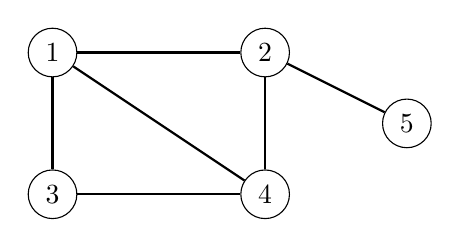
\begin{tikzpicture}[scale=0.9]
\node[draw, circle] (1) at (1,3) {$1$};
\node[draw, circle] (2) at (4,3) {$2$};
\node[draw, circle] (3) at (1,1) {$3$};
\node[draw, circle] (4) at (4,1) {$4$};
\node[draw, circle] (5) at (6,2) {$5$};

\path[draw,thick,-] (1) -- (2);
\path[draw,thick,-] (1) -- (3);
\path[draw,thick,-] (1) -- (4);
\path[draw,thick,-] (3) -- (4);
\path[draw,thick,-] (2) -- (4);
\path[draw,thick,-] (2) -- (5);
%\path[draw,thick,-] (4) -- (5);
\end{tikzpicture}
\end{center}

La suma de los grados en un grafo siempre es $2m$,
donde $m$ es el número de aristas,
porque cada arista
aumenta el grado de exactamente dos nodos en uno.
Por esta razón, la suma de los grados siempre es par.

\index{grafo regular}
\index{grafo completo}

Un grafo es \key{regular} si el
grado de cada nodo es una constante $d$.
Un grafo es \key{completo} si el
grado de cada nodo es $n-1$, es decir,
el grafo contiene todas las aristas posibles
entre los nodos.

\index{grado de entrada}
\index{grado de salida}

En un grafo dirigido, el \key{grado de entrada}
de un nodo es el número de aristas
que terminan en el nodo,
y el \key{grado de salida} de un nodo
es el número de aristas que comienzan en el nodo.
Por ejemplo, en el siguiente grafo,
el grado de entrada del nodo 2 es 2,
y el grado de salida del nodo 2 es 1.

\begin{center}
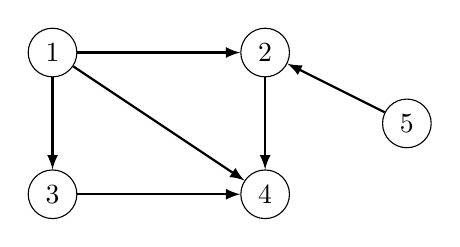
\begin{tikzpicture}[scale=0.9]
\node[draw, circle] (1) at (1,3) {$1$};
\node[draw, circle] (2) at (4,3) {$2$};
\node[draw, circle] (3) at (1,1) {$3$};
\node[draw, circle] (4) at (4,1) {$4$};
\node[draw, circle] (5) at (6,2) {$5$};

\path[draw,thick,->,>=latex] (1) -- (2);
\path[draw,thick,->,>=latex] (1) -- (3);
\path[draw,thick,->,>=latex] (1) -- (4);
\path[draw,thick,->,>=latex] (3) -- (4);
\path[draw,thick,->,>=latex] (2) -- (4);
\path[draw,thick,<-,>=latex] (2) -- (5);
\end{tikzpicture}
\end{center}

\subsubsection{Coloración}

\index{coloración}
\index{grafo bipartito}

En una \key{coloración} de un grafo,
a cada nodo se le asigna un color de tal manera que
no haya nodos adyacentes del mismo color.

Un grafo es \key{bipartito} si
es posible colorearlo usando dos colores.
Resulta que un grafo es bipartito
exactamente cuando no contiene un ciclo
con un número impar de aristas.
Por ejemplo, el grafo
\begin{center}
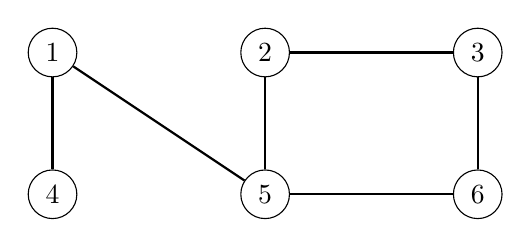
\begin{tikzpicture}[scale=0.9]
\node[draw, circle] (1) at (1,3) {$2$};
\node[draw, circle] (2) at (4,3) {$3$};
\node[draw, circle] (3) at (1,1) {$5$};
\node[draw, circle] (4) at (4,1) {$6$};
\node[draw, circle] (5) at (-2,1) {$4$};
\node[draw, circle] (6) at (-2,3) {$1$};
\path[draw,thick,-] (1) -- (2);
\path[draw,thick,-] (1) -- (3);
\path[draw,thick,-] (3) -- (4);
\path[draw,thick,-] (2) -- (4);
\path[draw,thick,-] (3) -- (6);
\path[draw,thick,-] (5) -- (6);
\end{tikzpicture}
\end{center}
es bipartito, porque se puede colorear de la siguiente manera:
\begin{center}
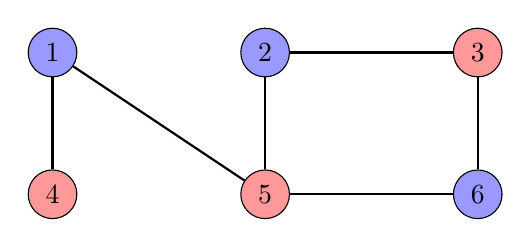
\begin{tikzpicture}[scale=0.9]
\node[draw, circle, fill=blue!40] (1) at (1,3) {$2$};
\node[draw, circle, fill=red!40] (2) at (4,3) {$3$};
\node[draw, circle, fill=red!40] (3) at (1,1) {$5$};
\node[draw, circle, fill=blue!40] (4) at (4,1) {$6$};
\node[draw, circle, fill=red!40] (5) at (-2,1) {$4$};
\node[draw, circle, fill=blue!40] (6) at (-2,3) {$1$};
\path[draw,thick,-] (1) -- (2);
\path[draw,thick,-] (1) -- (3);
\path[draw,thick,-] (3) -- (4);
\path[draw,thick,-] (2) -- (4);
\path[draw,thick,-] (3) -- (6);
\path[draw,thick,-] (5) -- (6);
\end{tikzpicture}
\end{center}
Sin embargo, el grafo
\begin{center}
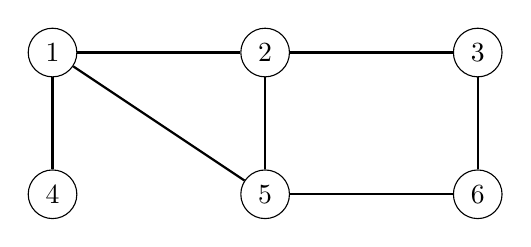
\begin{tikzpicture}[scale=0.9]
\node[draw, circle] (1) at (1,3) {$2$};
\node[draw, circle] (2) at (4,3) {$3$};
\node[draw, circle] (3) at (1,1) {$5$};
\node[draw, circle] (4) at (4,1) {$6$};
\node[draw, circle] (5) at (-2,1) {$4$};
\node[draw, circle] (6) at (-2,3) {$1$};
\path[draw,thick,-] (1) -- (2);
\path[draw,thick,-] (1) -- (3);
\path[draw,thick,-] (3) -- (4);
\path[draw,thick,-] (2) -- (4);
\path[draw,thick,-] (3) -- (6);
\path[draw,thick,-] (5) -- (6);
\path[draw,thick,-] (1) -- (6);
\end{tikzpicture}
\end{center}
no es bipartito, porque no es posible colorear
el siguiente ciclo de tres nodos usando dos colores:
\begin{center}
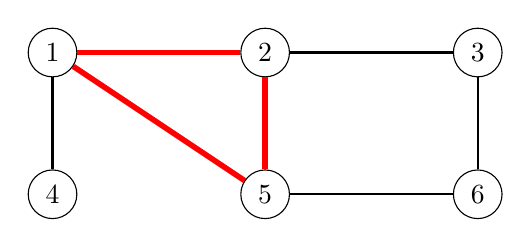
\begin{tikzpicture}[scale=0.9]
\node[draw, circle] (1) at (1,3) {$2$};
\node[draw, circle] (2) at (4,3) {$3$};
\node[draw, circle] (3) at (1,1) {$5$};
\node[draw, circle] (4) at (4,1) {$6$};
\node[draw, circle] (5) at (-2,1) {$4$};
\node[draw, circle] (6) at (-2,3) {$1$};
\path[draw,thick,-] (1) -- (2);
\path[draw,thick,-] (1) -- (3);
\path[draw,thick,-] (3) -- (4);
\path[draw,thick,-] (2) -- (4);
\path[draw,thick,-] (3) -- (6);
\path[draw,thick,-] (5) -- (6);
\path[draw,thick,-] (1) -- (6);

\path[draw=red,thick,-,line width=2pt] (1) -- (3);
\path[draw=red,thick,-,line width=2pt] (3) -- (6);
\path[draw=red,thick,-,line width=2pt] (6) -- (1);
\end{tikzpicture}
\end{center}

\subsubsection{Simplicidad}

\index{grafo simple}

Un grafo es \key{simple}
si ninguna arista comienza y termina en el mismo nodo,
y no hay múltiples
aristas entre dos nodos.
A menudo, asumimos que los grafos son simples.
Por ejemplo, el siguiente grafo \emph{no} es simple:
\begin{center}
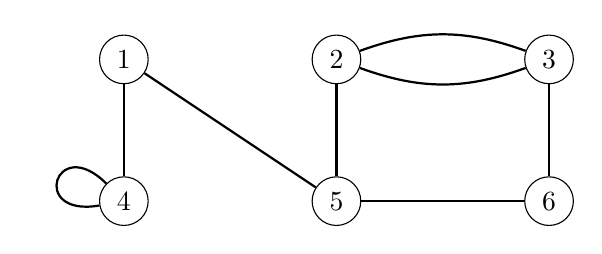
\begin{tikzpicture}[scale=0.9]
\node[draw, circle] (1) at (1,3) {$2$};
\node[draw, circle] (2) at (4,3) {$3$};
\node[draw, circle] (3) at (1,1) {$5$};
\node[draw, circle] (4) at (4,1) {$6$};
\node[draw, circle] (5) at (-2,1) {$4$};
\node[draw, circle] (6) at (-2,3) {$1$};

\path[draw,thick,-] (1) edge [bend right=20] (2);
\path[draw,thick,-] (2) edge [bend right=20] (1);
%\path[draw,thick,-] (1) -- (2);
\path[draw,thick,-] (1) -- (3);
\path[draw,thick,-] (3) -- (4);
\path[draw,thick,-] (2) -- (4);
\path[draw,thick,-] (3) -- (6);
\path[draw,thick,-] (5) -- (6);

\tikzset{every loop/.style={in=135,out=190}}
\path[draw,thick,-] (5) edge [loop left] (5);
\end{tikzpicture}
\end{center}

\section{Graph representation}

There are several ways to represent graphs
in algorithms.
The choice of a data structure
depends on the size of the graph and
the way the algorithm processes it.
Next we will go through three common representations.

\subsubsection{Adjacency list representation}

\index{adjacency list}

In the adjacency list representation,
each node $x$ in the graph is assigned an \key{adjacency list}
that consists of nodes
to which there is an edge from $x$.
Adjacency lists are the most popular
way to represent graphs, and most algorithms can be
efficiently implemented using them.

A convenient way to store the adjacency lists is to declare
an array of vectors as follows:
\begin{lstlisting}
vector<int> adj[N];
\end{lstlisting}

The constant $N$ is chosen so that all
adjacency lists can be stored.
For example, the graph

\begin{center}
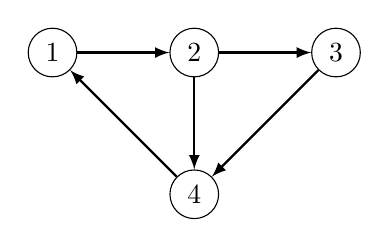
\begin{tikzpicture}[scale=0.9]
\node[draw, circle] (1) at (1,3) {$1$};
\node[draw, circle] (2) at (3,3) {$2$};
\node[draw, circle] (3) at (5,3) {$3$};
\node[draw, circle] (4) at (3,1) {$4$};

\path[draw,thick,->,>=latex] (1) -- (2);
\path[draw,thick,->,>=latex] (2) -- (3);
\path[draw,thick,->,>=latex] (2) -- (4);
\path[draw,thick,->,>=latex] (3) -- (4);
\path[draw,thick,->,>=latex] (4) -- (1);
\end{tikzpicture}
\end{center}
can be stored as follows:
\begin{lstlisting}
adj[1].push_back(2);
adj[2].push_back(3);
adj[2].push_back(4);
adj[3].push_back(4);
adj[4].push_back(1);
\end{lstlisting}

If the graph is undirected, it can be stored in a similar way,
but each edge is added in both directions.

For a weighted graph, the structure can be extended
as follows:

\begin{lstlisting}
vector<pair<int,int>> adj[N];
\end{lstlisting}

In this case, the adjacency list of node $a$
contains the pair $(b,w)$
always when there is an edge from node $a$ to node $b$
with weight $w$. For example, the graph

\begin{center}
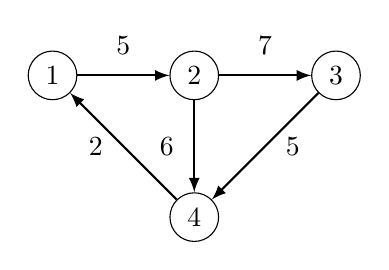
\begin{tikzpicture}[scale=0.9]
\node[draw, circle] (1) at (1,3) {$1$};
\node[draw, circle] (2) at (3,3) {$2$};
\node[draw, circle] (3) at (5,3) {$3$};
\node[draw, circle] (4) at (3,1) {$4$};

\path[draw,thick,->,>=latex] (1) -- node[font=\small,label=above:5] {} (2);
\path[draw,thick,->,>=latex] (2) -- node[font=\small,label=above:7] {} (3);
\path[draw,thick,->,>=latex] (2) -- node[font=\small,label=left:6] {} (4);
\path[draw,thick,->,>=latex] (3) -- node[font=\small,label=right:5] {} (4);
\path[draw,thick,->,>=latex] (4) -- node[font=\small,label=left:2] {} (1);
\end{tikzpicture}
\end{center}
can be stored as follows:
\begin{lstlisting}
adj[1].push_back({2,5});
adj[2].push_back({3,7});
adj[2].push_back({4,6});
adj[3].push_back({4,5});
adj[4].push_back({1,2});
\end{lstlisting}

The benefit of using adjacency lists is that
we can efficiently find the nodes to which
we can move from a given node through an edge.
For example, the following loop goes through all nodes
to which we can move from node $s$:

\begin{lstlisting}
for (auto u : adj[s]) {
    // process node u
}
\end{lstlisting}

\subsubsection{Adjacency matrix representation}

\index{adjacency matrix}

An \key{adjacency matrix} is a two-dimensional array
that indicates which edges the graph contains.
We can efficiently check from an adjacency matrix
if there is an edge between two nodes.
The matrix can be stored as an array
\begin{lstlisting}
int adj[N][N];
\end{lstlisting}
where each value $\texttt{adj}[a][b]$ indicates
whether the graph contains an edge from
node $a$ to node $b$.
If the edge is included in the graph,
then $\texttt{adj}[a][b]=1$,
and otherwise $\texttt{adj}[a][b]=0$.
For example, the graph
\begin{center}
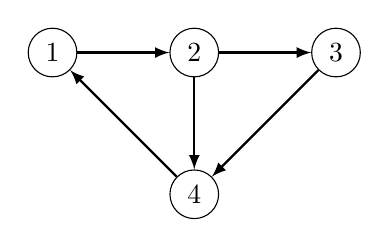
\begin{tikzpicture}[scale=0.9]
\node[draw, circle] (1) at (1,3) {$1$};
\node[draw, circle] (2) at (3,3) {$2$};
\node[draw, circle] (3) at (5,3) {$3$};
\node[draw, circle] (4) at (3,1) {$4$};

\path[draw,thick,->,>=latex] (1) -- (2);
\path[draw,thick,->,>=latex] (2) -- (3);
\path[draw,thick,->,>=latex] (2) -- (4);
\path[draw,thick,->,>=latex] (3) -- (4);
\path[draw,thick,->,>=latex] (4) -- (1);
\end{tikzpicture}
\end{center}
can be represented as follows:
\begin{center}
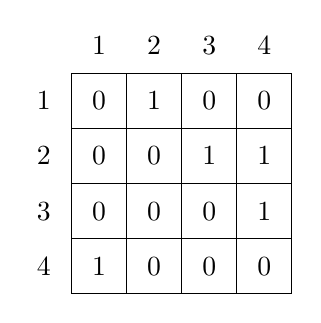
\begin{tikzpicture}[scale=0.7]
\draw (0,0) grid (4,4);
\node at (0.5,0.5) {1};
\node at (1.5,0.5) {0};
\node at (2.5,0.5) {0};
\node at (3.5,0.5) {0};
\node at (0.5,1.5) {0};
\node at (1.5,1.5) {0};
\node at (2.5,1.5) {0};
\node at (3.5,1.5) {1};
\node at (0.5,2.5) {0};
\node at (1.5,2.5) {0};
\node at (2.5,2.5) {1};
\node at (3.5,2.5) {1};
\node at (0.5,3.5) {0};
\node at (1.5,3.5) {1};
\node at (2.5,3.5) {0};
\node at (3.5,3.5) {0};
\node at (-0.5,0.5) {4};
\node at (-0.5,1.5) {3};
\node at (-0.5,2.5) {2};
\node at (-0.5,3.5) {1};
\node at (0.5,4.5) {1};
\node at (1.5,4.5) {2};
\node at (2.5,4.5) {3};
\node at (3.5,4.5) {4};
\end{tikzpicture}
\end{center}

If the graph is weighted, the adjacency matrix
representation can be extended so that
the matrix contains the weight of the edge
if the edge exists.
Using this representation, the graph

\begin{center}
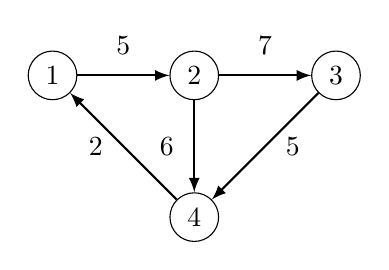
\begin{tikzpicture}[scale=0.9]
\node[draw, circle] (1) at (1,3) {$1$};
\node[draw, circle] (2) at (3,3) {$2$};
\node[draw, circle] (3) at (5,3) {$3$};
\node[draw, circle] (4) at (3,1) {$4$};

\path[draw,thick,->,>=latex] (1) -- node[font=\small,label=above:5] {} (2);
\path[draw,thick,->,>=latex] (2) -- node[font=\small,label=above:7] {} (3);
\path[draw,thick,->,>=latex] (2) -- node[font=\small,label=left:6] {} (4);
\path[draw,thick,->,>=latex] (3) -- node[font=\small,label=right:5] {} (4);
\path[draw,thick,->,>=latex] (4) -- node[font=\small,label=left:2] {} (1);
\end{tikzpicture}
\end{center}
\begin{samepage}
corresponds to the following matrix:
\begin{center}
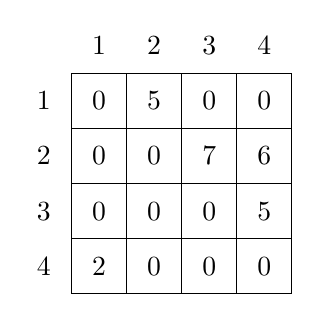
\begin{tikzpicture}[scale=0.7]
\draw (0,0) grid (4,4);
\node at (0.5,0.5) {2};
\node at (1.5,0.5) {0};
\node at (2.5,0.5) {0};
\node at (3.5,0.5) {0};
\node at (0.5,1.5) {0};
\node at (1.5,1.5) {0};
\node at (2.5,1.5) {0};
\node at (3.5,1.5) {5};
\node at (0.5,2.5) {0};
\node at (1.5,2.5) {0};
\node at (2.5,2.5) {7};
\node at (3.5,2.5) {6};
\node at (0.5,3.5) {0};
\node at (1.5,3.5) {5};
\node at (2.5,3.5) {0};
\node at (3.5,3.5) {0};
\node at (-0.5,0.5) {4};
\node at (-0.5,1.5) {3};
\node at (-0.5,2.5) {2};
\node at (-0.5,3.5) {1};
\node at (0.5,4.5) {1};
\node at (1.5,4.5) {2};
\node at (2.5,4.5) {3};
\node at (3.5,4.5) {4};
\end{tikzpicture}
\end{center}
\end{samepage}

The drawback of the adjacency matrix representation
is that the matrix contains $n^2$ elements,
and usually most of them are zero.
For this reason, the representation cannot be used
if the graph is large.

\subsubsection{Edge list representation}

\index{edge list}

An \key{edge list} contains all edges of a graph
in some order.
This is a convenient way to represent a graph
if the algorithm processes all edges of the graph
and it is not needed to find edges that start
at a given node.

The edge list can be stored in a vector
\begin{lstlisting}
vector<pair<int,int>> edges;
\end{lstlisting}
where each pair $(a,b)$ denotes that
there is an edge from node $a$ to node $b$.
Thus, the graph

\begin{center}
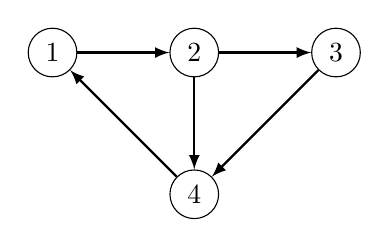
\begin{tikzpicture}[scale=0.9]
\node[draw, circle] (1) at (1,3) {$1$};
\node[draw, circle] (2) at (3,3) {$2$};
\node[draw, circle] (3) at (5,3) {$3$};
\node[draw, circle] (4) at (3,1) {$4$};

\path[draw,thick,->,>=latex] (1) -- (2);
\path[draw,thick,->,>=latex] (2) -- (3);
\path[draw,thick,->,>=latex] (2) -- (4);
\path[draw,thick,->,>=latex] (3) -- (4);
\path[draw,thick,->,>=latex] (4) -- (1);
\end{tikzpicture}
\end{center}
can be represented as follows:
\begin{lstlisting}
edges.push_back({1,2});
edges.push_back({2,3});
edges.push_back({2,4});
edges.push_back({3,4});
edges.push_back({4,1});
\end{lstlisting}

\noindent
If the graph is weighted, the structure can
be extended as follows:
\begin{lstlisting}
vector<tuple<int,int,int>> edges;
\end{lstlisting}
Each element in this list is of the
form $(a,b,w)$, which means that there
is an edge from node $a$ to node $b$ with weight $w$.
For example, the graph

\begin{center}
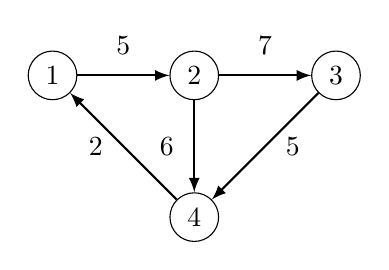
\begin{tikzpicture}[scale=0.9]
\node[draw, circle] (1) at (1,3) {$1$};
\node[draw, circle] (2) at (3,3) {$2$};
\node[draw, circle] (3) at (5,3) {$3$};
\node[draw, circle] (4) at (3,1) {$4$};

\path[draw,thick,->,>=latex] (1) -- node[font=\small,label=above:5] {} (2);
\path[draw,thick,->,>=latex] (2) -- node[font=\small,label=above:7] {} (3);
\path[draw,thick,->,>=latex] (2) -- node[font=\small,label=left:6] {} (4);
\path[draw,thick,->,>=latex] (3) -- node[font=\small,label=right:5] {} (4);
\path[draw,thick,->,>=latex] (4) -- node[font=\small,label=left:2] {} (1);
\end{tikzpicture}
\end{center}
\begin{samepage}
can be represented as follows\footnote{In some older compilers, the function
\texttt{make\_tuple} must be used instead of the braces (for example,
\texttt{make\_tuple(1,2,5)} instead of \texttt{\{1,2,5\}}).}:
\begin{lstlisting}
edges.push_back({1,2,5});
edges.push_back({2,3,7});
edges.push_back({2,4,6});
edges.push_back({3,4,5});
edges.push_back({4,1,2});
\end{lstlisting}
\end{samepage}
